\documentclass{beamer}
\usepackage{subfig}
\usepackage{xcolor}
\usepackage[utf8]{inputenc}
\hypersetup{
	colorlinks,
	allcolors= .,
	urlcolor = red,
	citecolor = black,
}
\usepackage{color}
\urlstyle{same}
\setbeamerfont{footnote}{size=\tiny}
\DeclareMathOperator*{\argmax}{arg\,max}
\DeclareMathOperator*{\argmin}{arg\,min}

% \usepackage{utopia} %font utopia imported
\usepackage[style=authortitle,backend=bibtex]{biblatex}
\addbibresource{references.bib}

\newcommand{\blue}[1]{{\color{blue} #1}}
\newcommand{\red}[1]{{\color{red} #1}}

\usetheme{Madrid}
\usecolortheme{default}
\title[] %optional
{Optimization-based Motion Planning and Optimal Control}

\author[Jun Zeng]{Jun Zeng}

\institute[UC Berkeley]
{
    Department of Mechanical Engineering \\
    University of California, Berkeley
}

\date[February 18th 2020]
{February 18th 2020}

\AtBeginSection[]
{
  \begin{frame}
    \tableofcontents[currentsection]
  \end{frame}
}

\begin{document}
%The next statement creates the title page.
\frame{\titlepage}

\begin{frame}
	\frametitle{Overview} 
	\tableofcontents
\end{frame}

\section{Introduction}
\begin{frame}{Optimal Control vs Optimization-based Path Planning}
	\begin{itemize}
		\item Optimal control: linear–quadratic regulator (LQR), model predictive control (MPC), sliding mode control, etc.
		\item Topics in optimization-based path planning:
		\begin{itemize}
			\item Speed profile smoothing: e.g. minimum-jerk in autonomous driving.
			\item Contact force: e.g. hybrid mode switch with contact force in legged robotics.
			\item Energy efficiency: e.g. minimum-snap/jerk in aerial robotics.
		\end{itemize} 
		\item They are the same in mathematics: an optimization problem is formulated to generate control strategy or trajectory/robot's motions.
		\item They are different in the implementation: optimal control is usually holding a higher refresh rate and needs to be solved very fast, while the  optimization problem in planning isn't necessarily to be solved computationally with that fast rate.
	\end{itemize}
\end{frame}

\begin{frame}{Notation}
	Generally, an optimal control problem or an optimization-based path planning problem could be described as follow,
	\begin{align*}
		u^*(t) :=& \argmin_{u(.)} \int_{t_0}^{t_f} c_t (x(t), u(t)) dt \\
		\textit{s.t.} \ & x(t_0) = x_0 \\
		& \dot{x}(t) = f(x(t), u(t)) \quad \forall t \\
		& x(t) \in \mathcal{X}_{feas} \quad \forall t \quad \text{(collision-free)} \\
		& u(t) \in \mathcal{U}_{feas} \quad \forall t \quad \text{(control limits)}
	\end{align*}
	\begin{itemize}
		\item In the view of control: generate feasible control inputs under dynamics constraints
		\item In the view of planning: generate dynamically-feasible waypoints (which will be tracked with appropriate control methods).
	\end{itemize}
\end{frame}

\section{Optimization-based path planning}
\subsection{General methods}
\begin{frame}{Mathematical methods}
	Generally, a optimization problem will satisfy a variety of constraints, this leads us to have different methods to solve them numerically.
	
	Some of them have explicit solutions:
	\begin{itemize}
		\item convex quadratic programming (Convex QP)
		\item LQR: For continuous-system linear system $\dot{x} = Ax + Bu$ with a quadratic cost
		$J = \int_0^{\infty} (x^T Q x + u^T R u + 2x^T N u) dt$. The feedback control law to minimize the value of the cost is $u = -Kx$, where $K = R^{-1} (B^T P + N^T)$ and $A^T P + P A - (P B + N) R^{-1} (B^T P + N^T) + Q = 0$. Here, the control law could be solved \red{explicitly}. 
	\end{itemize}
\end{frame}

\begin{frame}{Numerical methods}
	Other general problems don't have explicit solutions and don't guarantee existing solution but could be solved numerically:
	
	An optimization-based path planning problem could be formulated as several types:
	\begin{itemize}
		\item Shooting methods: we 'shoot' out trajectories in different directions until we find a trajectory that has the desired boundary value.
		\item Collocation methods: choose a finite-dimensional space of candidate solutions (e.g. polynomials) and a number of points in the domain (called collocation points), and to select that solution which satisfies the given equation at the collocation points.
	\end{itemize}
\end{frame}

\begin{frame}{Solvers and existence of solutions}
	Most likely, all problems could be formulated into a dynamic programming problem and could be solved with various numerical solvers\footnote{More mathematical details for solving optimization problem are presented in EE 227A/B/C.}:
	\begin{itemize}
		\item for convex problems:
		\begin{itemize}
			\item software: CVX, OSQP
			\item internal solvers: Gurobi, Sedumi, Mosek  
		\end{itemize}
		\item for non-convex problems:
		\begin{itemize}
			\item interior point: IPOPT, SNOPT
			\item active set method: SAS
		\end{itemize}
	\end{itemize}
	\vspace{\baselineskip}

	We are more interested in the existence of the solution of the optimization. For a convex problem, we are likely to ensure at least one solution (might have several ones if it's nonlinear or non-convex cost function, our numerical solution will depends on the initial point where we do gradient descent). But for general non-convex problem, we are \red{unable to} guarantee the existence of solution. 
\end{frame}

\subsection{Examples}
\begin{frame}{Trajectory smoothing}
	One of the most applicable areas about optimization-based planning is trajectory smoothing, which intends to make trajectory generated from the sample-based methods (RRT, PRM, etc) become smoother.
	\begin{figure}
		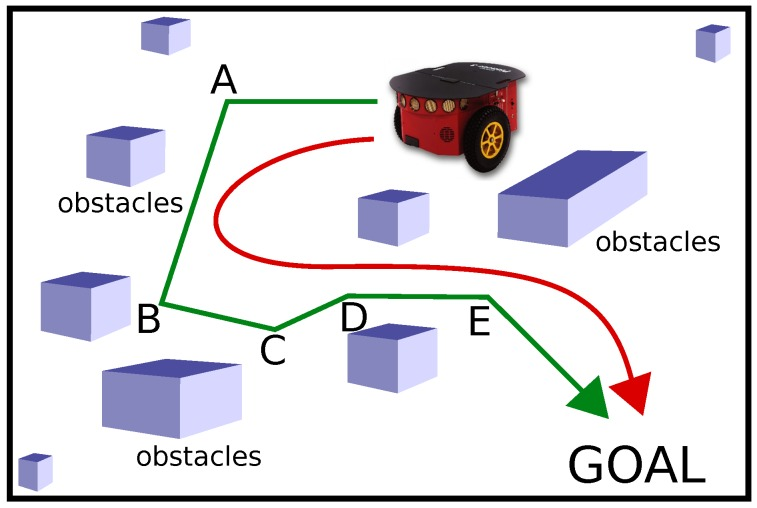
\includegraphics[width=0.5\linewidth]{figures/trajectory-smooth.jpg}
		\caption{Make your trajectory smoother}
	\end{figure}
\end{frame}

\begin{frame}{Geometric interpolation}
	There are some traditional geometric methods for trajectory smoothing:
	\begin{itemize}
		\item Polynomial interpolation
		\item Bezier Curve \href{https://www.geogebra.org/m/r3UWE9KR}{[online playground]}
		\item Cubic Splines
		\item B-Splined
	\end{itemize}
	\begin{figure}
		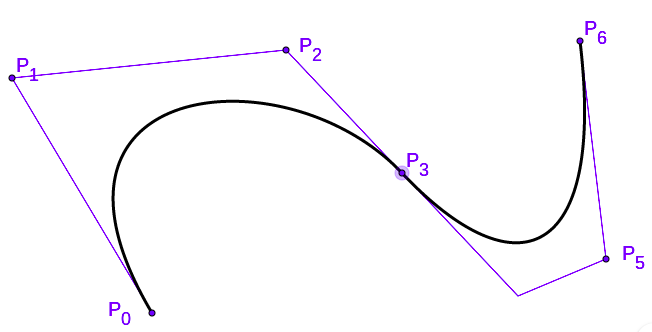
\includegraphics[width=0.5\linewidth]{figures/bezier_curve.png}
		\caption{Bezier Curve}
	\end{figure}
\end{frame}

\begin{frame}{Special curves for smoothness}
	In industry, people prefer some special curves which are easy to be implemented with less complexity:
	\begin{itemize}
		\item Dubin’s Curve (e.g. lane change in autonomous driving)
		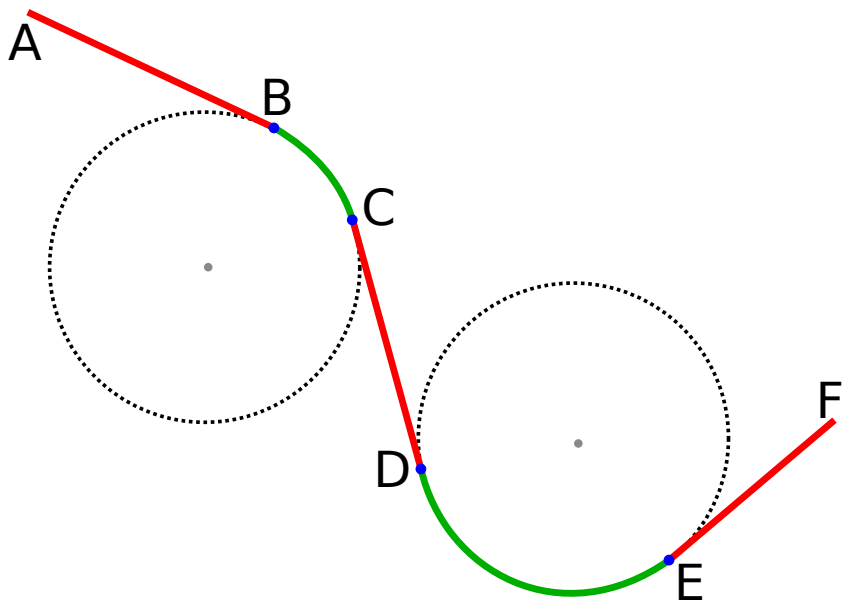
\includegraphics[width=0.5\linewidth]{figures/dubin-curve.png}
	\end{itemize}
\end{frame}

\begin{frame}{Optimization-based methods}
	The optimization-based methods could also deal with trajectory smoothing problem. For example, minimum-time for obstacle avoidance \footcite{hauser2010fast}.
	\begin{figure}
		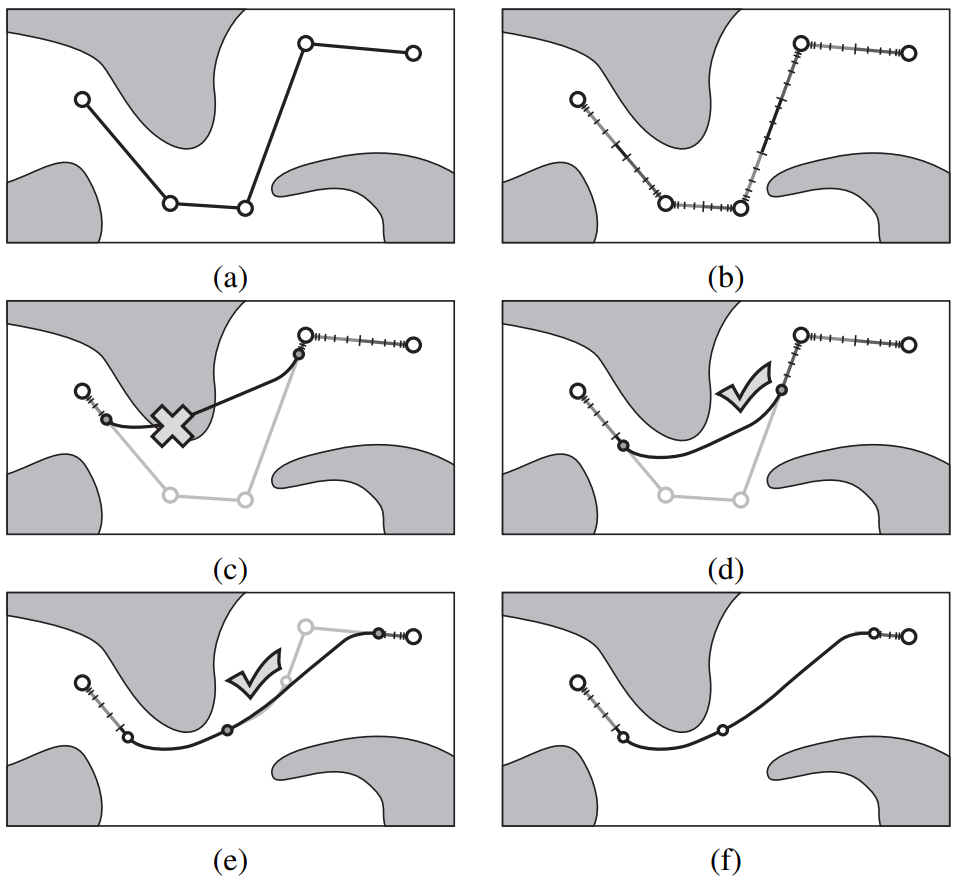
\includegraphics[width=0.4\linewidth]{figures/trajectory-smooth-optimal-bounded-acceleration.png}
	\end{figure}
	Here, only bounded acceleration is considered, dynamics is still excluded.
\end{frame}

\begin{frame}{Related work}
	\begin{itemize}
		\item "Time Elastic Band" planner (TEB Planner) with ROS integration is introduced \footcite{rosmann2012trajectory} \footcite{rosmann2013efficient}, where non-holonomic kinematics is considered, but roughtly. \href{https://www.youtube.com/watch?v=e1Bw6JOgHME&feature=emb_title}{[demo video in ROS]}
		\item Some receding horizon methods are also introduced \footcite{kogan2006optimization}.
		\item For autonomous driving, some special techniques are also proposed \footcite{dolgov2010path} \footcite{ziegler2014trajectory} \footcite{gu2012road}.
	\end{itemize}
\end{frame}

\begin{frame}
	There are many work about this area, the pipeline of path planning is mainly considered as trajectory generation + trajectory smooth, and the problem is formulated to consider mobile robots not holding too complex dynamics (autonomous cars, robot arm, etc).
	
	\vspace{\baselineskip}
	How about generating a dynamically-feasible trajectory directly from an optimization-based problem? There are several tricky points to take into account.
	\begin{itemize}
		\item Obstacle avoidance
		\item Hybrid mode switch (contact force)
		\item Energy efficiency and smoothness (e.g. which kind of cost function we shall choose)
	\end{itemize}
\end{frame}

\begin{frame}{Obstacle avoidance}
	There are several ways to consider obstacle avoidance as constraints in an optimization-based problem:
	\begin{itemize}
		\item simple geometric constraints: e.g. $(x - x_{obs})^2 + (y - y_{obs})^2 \geq r^2 $
		\begin{itemize}
			\item very rough consideration: point-mass and round obstacle
			\item nonlinear and non-convex constraints
			\item it could be solved with modern solvers (IPOPT, etc) but doesn't guarantee a solution. 
		\end{itemize}
	\end{itemize}
\end{frame}

\begin{frame}{Obstacle avoidance}
	To make the problem become convex, an mixed-integer formulation could be introduced \footcite{richards2002aircraft} \footcite{deits2014footstep} \footcite{deits2015efficient}, which exploits the topological property of the collision-free space. We call it as "mixed-integer", since a list of integer variables is to used to represent the areas where the mobile robot is optimized to pass through. 
	\begin{figure}
		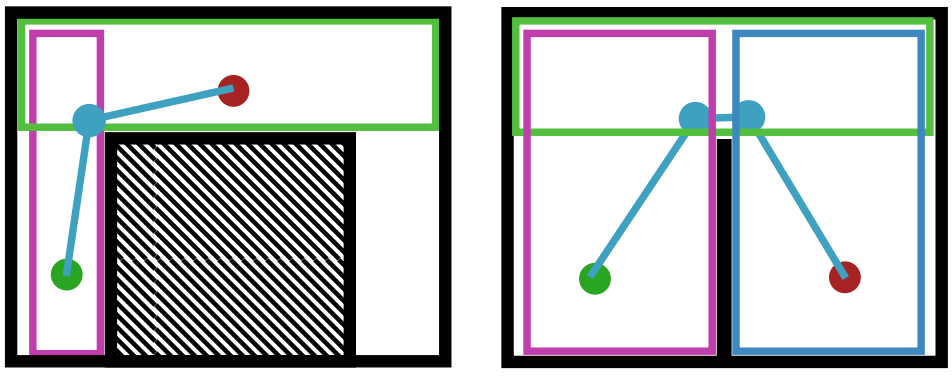
\includegraphics[width=0.5\linewidth]{figures/collision-free-mixed-integer.png}
		\caption{A trajectory in which each linear segment is required to remain entirely within one of the convex obstacle-free regions indicated by the colored boxes. This requirement ensures that the entire trajectory is collision-free.}
	\end{figure}
\end{frame}

\begin{frame}{Obstacle avoidance}
	Sometime we need to describe our robot and obstacles as rigid bodies, this leads us to define the distance between rigid body and obstacle avoidance constraint between them. \href{https://raw.githubusercontent.com/XiaojingGeorgeZhang/OBCA/master/images/TrajBack_ParkingVideo.gif}{[demo]}
	\begin{figure}
		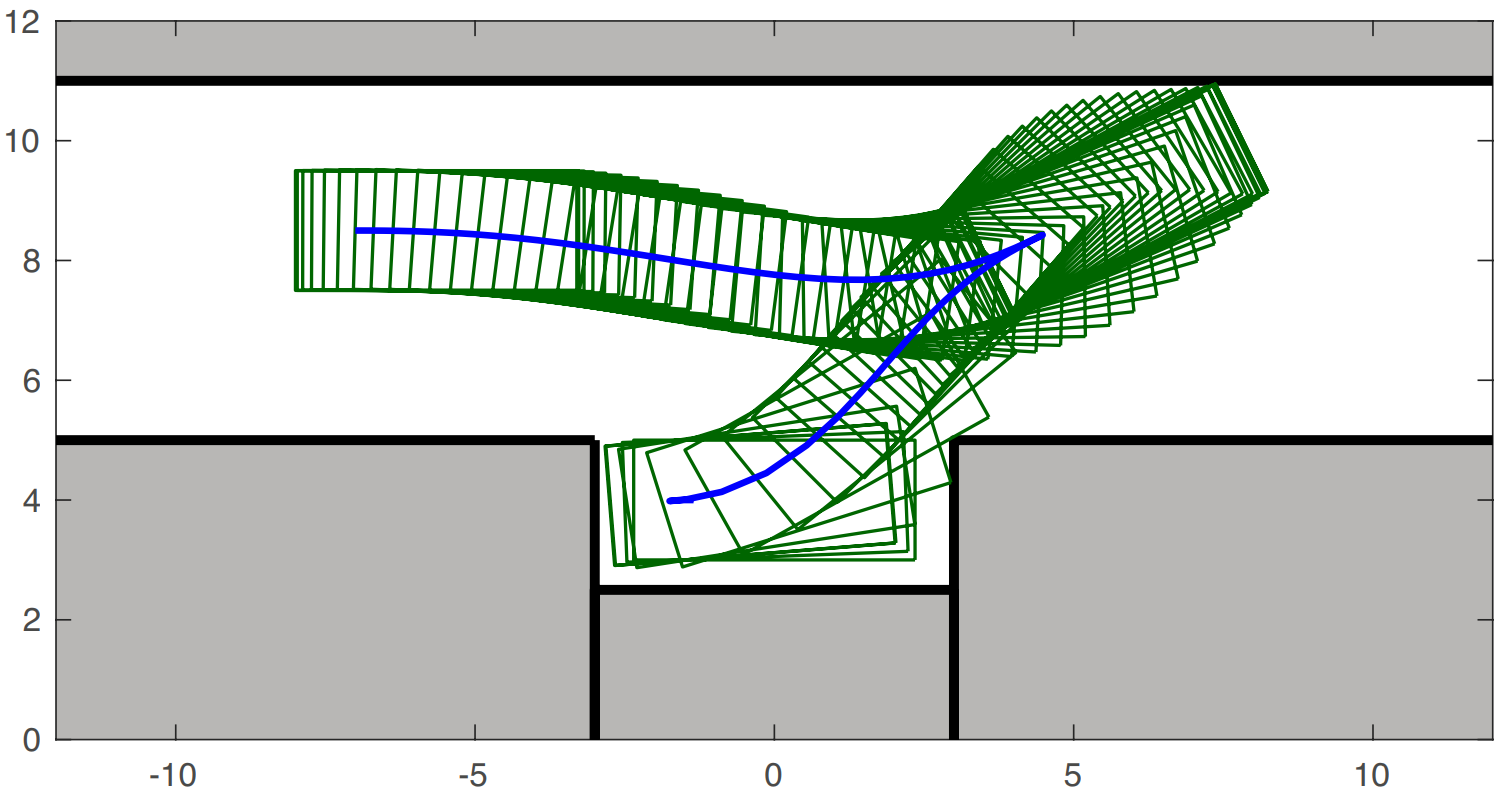
\includegraphics[width=0.5\linewidth]{figures/parallel-parking.png}
		\caption{Dual variables are used to represent the collision-free constraints, see more details in \footcite{zhang2017optimization}.}
	\end{figure}
\end{frame}

\begin{frame}{Contact force}
	The intuition is simple: contact force is zero or distance between contact points should be zero. This formulates a complementarity constraint.
	
	\vspace{\baselineskip}
	Generally, the methods is called \emph{Optimization through contact \footcite{posa2014direct}} and the problem is formulated as,
	\begin{align*}
		\text{find} \ & \ddot{q}, \lambda \\
		\text{subject to} \ & H(q) \ddot{q} + C(q, \dot{q}) + G(q) = B(q) u + J(q)^T \lambda \\
		& \phi(q) \geq 0 \\
		& \lambda \geq 0 \\
		& \phi(q)^T \lambda  = 0
	\end{align*}
	where $\lambda$ represents the contact force.
\end{frame}

\begin{frame}{Contact force}
	For example, the tension $T(t)$ in a massless cable could be considered as a contact force. Assume the length of cable is $l_0$ and the distance between two ends of the cable is $l(t)$, then we have $\phi(q) = l_0 - l(t) \geq 0$ with its complementarity constraint,
	\begin{equation*}
	T(t) (l_0 - l(t)) = 0
	\end{equation*}
	\begin{figure}
		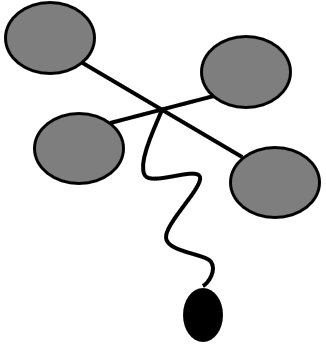
\includegraphics[width=0.2\linewidth]{figures/aerial-manipulation.png}
		\caption{Aerial manipulation: quadrotor with a suspended point-mass payload is a hybrid system, where the cable could be taut or slack.}
	\end{figure}
\end{frame}

\begin{frame}{Energy efficiency and smoothness}
	\begin{itemize}
		\item A cost function to minimize jerk (third-order derivative of vehicle's position) \footcite{pattacini2010experimental}.
		\item A cost function to minimize snap (fourth-order derivative of vehicle's position) \footcite{mellinger2011minimum}.
	\end{itemize}

	Actually, people find that minimum jerk or snap usually performed better than those of other orders in robots for smoothness. 
\end{frame}

\begin{frame}{Discussion}
	The optimization-based path planning is still active research topic, there are many existing problems which need to be solved:
	\begin{itemize}
		\item multi-agents: e.g. ensure collision-free movements in drone swarm
		\item safety: e.g. guarantee safety-critical trajectory in a noisy environment (sensor noise, model uncertainty, algorithm bias, etc)
		\item policy: centralized/decentralized, human-robot interaction
	\end{itemize}
	
\end{frame}

\section{Optimal control}
\subsection{Model predictive control}
\begin{frame}{Linear–quadratic regulator (LQR)}
	The LQR algorithm reduces the amount of work done by the control systems engineer to optimize the controller.
	\begin{align*}
		J^* &= \min_{u_i} \sum_{k = 0}^{N} x_{k+1}^T Q x_{k+1} + u_k^T R u_k \\
		\text{s.t.} \ & x_{k+1} = A x_{k} + B u_{k}
	\end{align*}
	There is no \emph{prediction} here, feedback control gain is constant here.
\end{frame}


\begin{frame}{Receding horizon control}
	Let's present model prediction control as follow,
	\begin{align*}
		J_t^*(x(t)) &= p(x_{t+N}) + \sum_{k = 0}^{N-1} q(x_{t+k}, u_{t+k}) \\
		\text{s.t.} &= x_{t+k+1} = A x_{t+k} + B u_{t+k}, k = 0,...,N-1 \\
		& x_{t+k} \in \mathcal{X}, u_{t+k} \in \mathcal{U}, k = 0,...,N-1 \\
		& x_{t+N} \in \mathcal{X}_f \\
		& x_t = x(t)
	\end{align*}
	Truncate after a finite horizon:
	\begin{itemize}
		\item $N$: horizon
		\item $p(x_{t+N})$: terminal cost which approximate the 'tail' of the cost.
		\item $q(x_{t+k}, u_{t+k})$: staged cost
		\item $\mathcal{X}_f$: Approximates the ‘tail’ of the constraints.
	\end{itemize}
\end{frame}

\begin{frame}{Model Predictive Control}
	\begin{figure}
		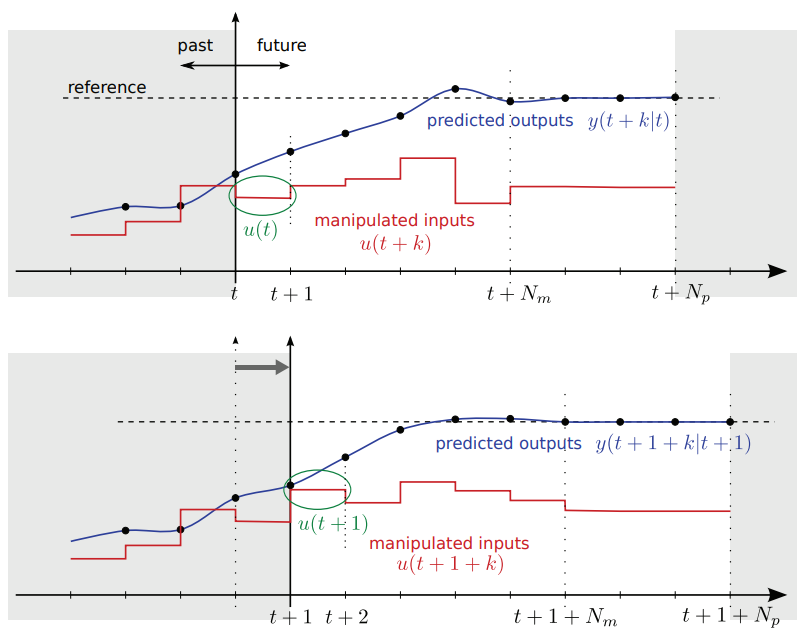
\includegraphics[width=0.5\linewidth]{figures/mpc-prediction.png}
	\end{figure}
	Where are the \emph{Predictions}?
	\begin{itemize}
		\item At each sampling time, solve a constrainted optimal control problem.
		\item Apply the optimal input only during $[t, t+1]$.
		\item At $t + 1$, solve a CFTOC over a shifted horizon based on new state measurements.
	\end{itemize}
\end{frame}

\begin{frame}{Open-loop vs Closed-loop }
	Some definitions among researchers working on MPC:
	\begin{itemize}
		\item Open-loop trajectory: at each time step, we have a constrainted optimal control problem, which solves a feasible trajectory with predictions.
		\item Closed-loop trajectory: since we solve optimal control problem at each time step, the robot will moves along a closed-loop trajectory with this control policy.
	\end{itemize}
\end{frame}

\begin{frame}{Discussions}
	\begin{itemize}
		\item Terminal cost ensures the Lyapunov convergence, but it's not necessary.
		\item Larger horizon brings a bigger controllable set, but needs more time to calculate the optimization.
		\item The dynamics constraints could be nonlinear, which will make the problem as a dynamic programming problem.
		\item There are many variants of MPC: Robust MPC, Adaptive MPC, MPC with obstacle avoidance, etc.
	\end{itemize}
\end{frame}




%\begin{frame}{References}
%	\printbibliography
%\end{frame}
\end{document}